% This report template is adapted from the IEEE style.
% https://www.ieee.org/conferences/publishing/templates.html

\documentclass[conference]{IEEEtran}
\IEEEoverridecommandlockouts

\usepackage{cite}
\usepackage{amsmath,amssymb,amsfonts}
\usepackage{algorithmic}
\usepackage{graphicx}
\usepackage{textcomp}
\usepackage{xcolor}
\usepackage{tikz}
\usepackage{hyperref}
\usepackage{float}
\def\BibTeX{{\rm B\kern-.05em{\sc i\kern-.025em b}\kern-.08em
    T\kern-.1667em\lower.7ex\hbox{E}\kern-.125emX}}

\begin{document}

\title{Towards Language Model-based Identification of Market Segments and Fostering of Business Clusters}

\author{\IEEEauthorblockN{1\textsuperscript{th} Müller Nicola}
\IEEEauthorblockA{s8namuel@stud.uni-saarland.de \\ 2578753}
\and
\IEEEauthorblockN{2\textsuperscript{st} Leist Robert}
\IEEEauthorblockA{s8roleis@stud.uni-saarland.de \\ 2580448}
\and
\IEEEauthorblockN{3\textsuperscript{nd} Eichler Paul}
\IEEEauthorblockA{s8pleich@stud.uni-saarland.de \\ 2578569}
\and
\IEEEauthorblockN{4\textsuperscript{rd} Recktenwald Tobias}
\IEEEauthorblockA{s8tsreck@stud.uni-saarland.de \\ 2577468}
\and
\IEEEauthorblockN{5\textsuperscript{th} Nazari Hameed}
\IEEEauthorblockA{Email Address \\ Matriculation No.}
}

\maketitle

\begin{abstract}
With this guide, we give an example of what a write-up for the mini-project report could look like. We provide a \LaTeX template that you 
can use in your own write-up, if you want to. We explain some important points regarding specific types of sections that need to be included in the report.
\end{abstract}


\section{Introduction}
\color{red} 
I need the business guys to check the following paragraph!
\color{black}

Identifying market segments in regional economies is crucial for effective marketing strategies and making well-informed business decisions. Further, combining geographical data of companies' locations with information on their corresponding market segments allows for detecting business clusters, which are local concentrations of businesses, manufacturers, suppliers, and institutions from the same field. This geographic proximity of related businesses enables efficient cooperation and knowledge transfer, which has been shown to significantly increase the productivity of all businesses within the cluster (citation). Thus, establishing or further developing business clusters is of high interest to companies and local governments.

However, the identification of market segments, and moreover that of business clusters, is complicated by the fact that data on regional companies is often unavailable or difficult to analyze due to non-numerical, irrelevant, or missing features.

This work demonstrates how to identify market segments and develop business clusters by introducing an automatic clustering pipeline and location recommendation system for economic data from the German federal state Saarland.

Our clustering pipeline can be divided into $4$ distinct steps: $1)$ gathering data from the websites of companies in Saarland, $2)$ computing embeddings of the data, $3)$ reducing the embeddings' dimensionality, and $4)$ applying clustering algorithms.

$1)$ To construct data points for companies in Saarland, we rely on publicly available descriptions from their websites, allowing us to circumvent the challenges of gathering economic data. Since these descriptions are intended to attract customers and investors, they contain all relevant information for characterizing the companies.

$2)$ Given the company descriptions, we utilize state-of-the-art language models to compute embeddings of the text data, corresponding to low-dimensional vectors encompassing the data's essential information. 

$3)$ We further reduce the dimensionality of the embeddings using non-linear dimensionality reduction techniques, which enables us to preserve the non-linear relationships between the embedded text data while avoiding the curse of dimensionality. 

$4)$ Lastly, we apply well-established clustering algorithms in the low-dimensional feature space to assign each company to a cluster corresponding to a potential market segment.

Our location recommendation system builds upon the clustering pipeline by computing an embedding of a novel company's description, assigning it to a cluster, and then identifying the most similar companies within the cluster. The system then recommends that the novel company locate its site near an established company acting in the same market segment, which fosters business cluster development in Saarland.

We provide a graphical user interface for our methods, which visualizes the clustering of companies in Saarland and their locations in an interactive manner, allowing end-users to analyze the various market segments. Further, the interface supports making location recommendations for new company sites using text inputs.

In summary, our main contributions are:
\begin{itemize}
    \item We circumvent the challenges of traditional economic data collection by relying solely on publicly available company descriptions.
    \item We leverage state-of-the-art language models to apply clustering algorithms to the high-dimensional text data.
    \item We demonstrate our approach's feasibility using Saarland's economy.
    \item We provide a user-friendly graphical interface for our methods, allowing for analyzing market segments and location recommendations for establishing business clusters.
\end{itemize}

The remaining parts of this paper are structured as follows: In section \MakeUppercase{\romannumeral 2}, we first examine the economy in Saarland and the theory behind business clusters. Then we look upon existing work on using clustering for economic analysis, and lastly, we investigate work on language models for extracting information from text. Next, in section \MakeUppercase{\romannumeral 3}, we present our methods in more detail, discussing each step of our clustering pipeline and location recommendation system, and in \MakeUppercase{\romannumeral 4}, we present how we apply our methods to the economy of Saarland. Lastly, we examine our results in section \MakeUppercase{\romannumeral 5} and conclude this work in section \MakeUppercase{\romannumeral 6}.

\section{Related Work}
\color{red}
\begin{itemize}
    \item General stuff about Saarland's economy and its market segments?
    \item How market segments are normally identified?
    \item Theory behind business clusters and maybe related work?
    \item Related Work on clustering in economy?
    \item Mention that we collected traditional economic data?
\end{itemize}
\color{black}

In natural language processing (NLP), translating text data to machine-processable representations is a fundamental challenge for numerous tasks, such as machine translation~\cite{qi2018and}, sentiment analysis~\cite{rezaeinia2019sentiment}, and information retrieval~\cite{ye2016word}, due to the complexity and variability of natural language. A popular approach for representing text data is the utilization of so-called \emph{embeddings}: vectorized representations of text with the property that vectors of text data with similar semantic and syntactic properties will have a smaller distance to vectors of text data with different properties. Thus, embeddings enable quantifying semantic and syntactic similarity in terms of distances in a low-dimensional, dense vector space, making them ideal for applying clustering to our sparse dataset of high-dimensional company descriptions.  

In general, embeddings are learned by training a neural network to perform a task requiring understanding semantic and syntactic information, such as predicting words given their surrounding contexts or predicting subsequent words in sentences. In this process, the network learns a mapping from its text input to low-dimensional representations, containing the information needed to generate correct outputs. Hence, the outputs of this mapping encode all relevant semantic and syntactic information in the text inputs, meaning that, after training, the network's corresponding layers can be reused to compute embeddings for other downstream tasks.

Mikolov et al~\cite{mikolov2013efficient}. popularized learning word embeddings from raw text data in $2013$ by introducing their Word2Vec model. GloVe, developed by Pennington et al.~\cite{pennington2014glove}, improved upon Word2Vec by effectively encoding both local context information and global statistical information into the embeddings, thereby offering more detailed semantic capture. More recently, transformer-based models like BERT, developed by Devlin et al.~\cite{devlin2018bert}, and GPT models by OpenAI~\cite{radford2018improving} have leveraged context-dependent word embeddings by encoding the words themselves and the context in which they are used. So-called sentence transformers extended these approaches by computing embeddings for entire sentences to capture more contextual information than individual word embeddings. Reimers and Gurevych~\cite{reimers2019sentence} introduced the Sentence-BERT model consisting of two Siamese BERT-networks, i.e., two BERT-networks with tied weights, which compute sentence embeddings by embedding each word individually and then applying a pooling layer calculating the maximum or mean over all word embeddings. Starting with pre-trained BERT-networks, Sentence-BERT is fine-tuned using text classification or cosine-similarity tasks, yielding a model capable of generating high-quality sentence embeddings using only a fraction of the original BERT model's computational effort.

\section{Procedure}
\begin{figure}[H]
    \centering
    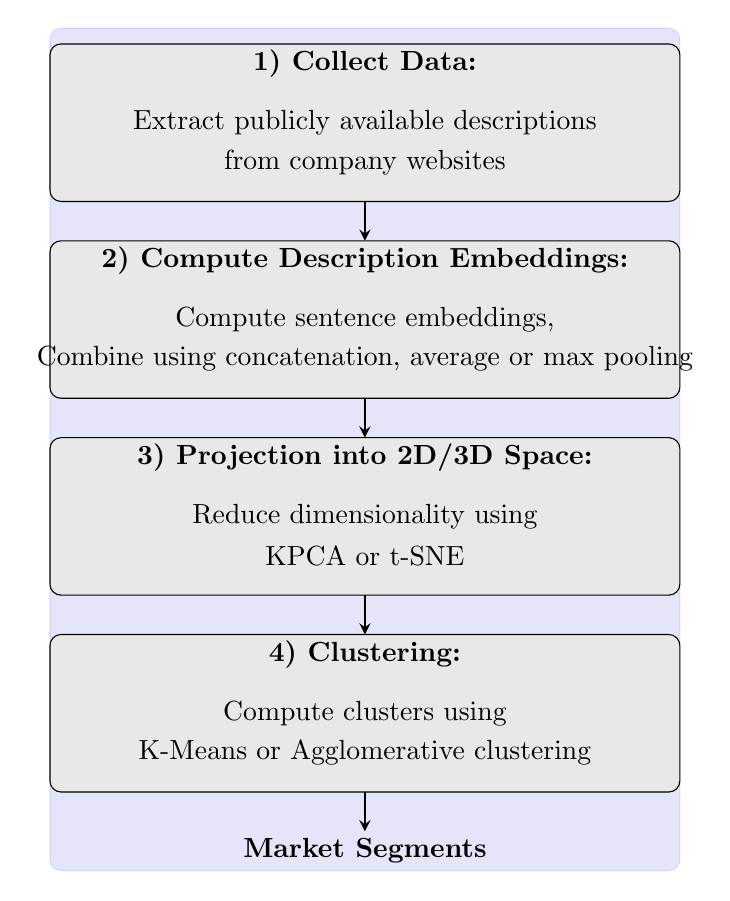
\begin{tikzpicture}
        \definecolor{lightgrey}{RGB}{232,232,232}
        \definecolor{darkblue}{RGB}{0,0,204}
        
        \draw[rounded corners, darkblue, fill=darkblue, opacity=0.1] (-4, -1) rectangle (4, 9.7);
    
        \draw[rounded corners, fill=lightgrey] (-4,7.5) rectangle (4, 9.5);
        \node[font=\bfseries] at (0, 9.25) {1) Collect Data:};
        \node at (0, 8.5) {Extract publicly available descriptions};
        \node at (0, 8.0) {from company websites};
        \draw[thick, -stealth] (0, 7.5) -- (0, 7);
    
        \draw[rounded corners, fill=lightgrey] (-4,5) rectangle (4, 7);
        \node[font=\bfseries] at (0, 6.75) {2) Compute Description Embeddings:};
        \node at (0, 6) {Compute sentence embeddings,};
        \node at (0, 5.5) {Combine using concatenation, average or max pooling};
        \draw[thick, -stealth] (0, 5) -- (0, 4.5);

        \draw[rounded corners, fill=lightgrey] (-4,2.5) rectangle (4, 4.5);
        \node[font=\bfseries] at (0, 4.25) {3) Projection into 2D/3D Space:};
        \node at (0, 3.5) {Reduce dimensionality using};
        \node at (0, 3.0) {KPCA or t-SNE};
        \draw[thick, -stealth] (0, 2.5) -- (0, 2);

        
        \draw[rounded corners, fill=lightgrey] (-4,0) rectangle (4, 2);
        \node[font=\bfseries] at (0, 1.75) {4) Clustering:};
        \node at (0, 1) {Compute clusters using};
        \node at (0, 0.5) {K-Means or Agglomerative clustering};
        \draw[thick, -stealth] (0, 0) -- (0, -0.5); 

        \node[font=\bfseries] at (0, -0.75) {Market Segments};
    \end{tikzpicture}
    \caption{Overview of our clustering pipeline.}
    \label{fig:pipeline}
\end{figure}
\pe{ s/Market Segments/Local Clusters; Market segment seems to be defined as segmenting your customer base \href{https://en.wikipedia.org/wiki/Market_segmentation}{wiki market segmentation}}



Our goal is to collect data points on companies in Saarland and cluster them to identify market segments and recommend locations for companies who plan to establish new sites, such that it supports the development of business clusters. We will present our clustering pipeline and then examine how we can use the results to provide location recommendations. 

\subsection{Identifying Market Segments through Clustering}
Figure \hyperref{fig:pipeline}{$1$} shows a graphical representation of our clustering pipeline, consisting of $4$ steps: $1)$ Collection of descriptions from company websites, $2)$ converting the descriptions to embeddings, $3)$ reducing the dimensionality of the embeddings, and $4)$ applying a clustering algorithm. In the following, we will examine each of these steps in detail.

\textit{$1)$ Collect Descriptions:} Given that high-quality economic data is highly valuable, there are no freely available data sets we could rely on for our purposes, meaning we need to build our dataset from scratch. The traditional approach for building such a dataset would be to gather several attributes, like revenue, number of employers, and products, for many companies in Saarland and then store each in a fixed-size vector. However, this approach has several drawbacks: It is not straightforward to encode non-numerical attributes, like products and customer base, such that clustering algorithms can parse them without introducing an unwanted ordering of the attributes' values. Further, some attributes may be unavailable for some companies, meaning we would need to discard them because we require fixed-size vectors, or we would need to insert dummy values, which could lead to unwanted effects. Lastly, representing a company using a small number of publicly available attributes might be insufficient for capturing all relevant characteristics. For instance, consider the smartphone manufacturers Apple and Samsung: Both companies build smartphones, have over $100.000$ employees, have revenues of over $200$ billion dollars, and have production and sales sites worldwide. Given these attributes, one could argue that Apple and Samsung are very similar companies. Yet, it is commonly known that Apple, with its minimalist design, high-end smartphones targeted toward customers looking to differentiate themselves from other people, and Samsung, with its more utilitarian smartphones targeted toward a broad customer base, are companies with fundamentally different characters.
To address these challenges to dataset construction, we propose representing companies by the description on their websites instead of numerical attributes. Since companies want to present themselves publicly in a way that attracts customers and investors, these descriptions contain the information needed to represent them accurately. 

\textit{$2)$ Compute Description Embeddings:} To achieve the fixed-size inputs required by clustering algorithms, we map each company description to an embedding that describes the data in a low-dimensional space. We rely on a sentence transformer neural network architecture to compute embeddings for each sentence in a company's description. We propose two approaches to get a single embedding for each description: we repeatedly concatenate individual sentence embeddings until a fixed size is achieved, or we take the maximum over each feature dimension. The first approach, which we will call padding, preserves each sentence embedding's information but may introduce bias and high dimensionality, whereas the second approach, which we will call max pooling, achieves a lower dimensionality but may discard relevant information by only keeping the largest features.

\textit{$3)$ Projection into 2D Space:} Although the embeddings are of much lower dimensionality than the original text data, the number of features might still be too large relative to the size of our dataset. This might invoke the curse of dimensionality, meaning that the few data points are so distant from each other in the high-dimensional space that it is impossible to derive meaningful clusters. Further, clustering data in high-dimensional space prevents the visualization of clustered data points. To avoid the course of dimensionality and to enable user-friendly visualization of our results, we will project the embeddings to 2D space using two dimensionality reduction techniques.
\emph{Kernel Principal Components Analysis} (KPCA) is a dimensionality reduction technique that computes a linear transformation that projects the data in the kernel space onto the dimensions with the highest variance, such that a non-linear transformation in the original feature space is attained. Hence, by projecting the data on the dimensions with the highest variance, KPCA preserves the most relevant information.
The \emph{t-distributed stochastic neighbor embedding} (t-SNE) technique computes a probability distribution representing the pairwise similarity between data points in the feature space and then projects the data points to a low-dimensional space according to a second probability distribution that minimizes the Kullback-Leibler divergence to the first distribution. This enables t-SNE to preserve local structures in the data accurately.
The crucial difference between KPCA and t-SNE is that KPCA computes a deterministic projection that can be applied to novel data points, whereas t-SNE does not. However, the preservation of local structures by t-SNE might be more suitable for identifying clusters.

\textit{$4)$ Clustering:} We will now present two clustering approaches that depend on the choice of dimensionality reduction technique.
If KPCA is used, we cluster the data using the $K$-Means algorithm, which, starting from $K$ randomly initialized cluster centers, assigns each data point to the nearest cluster, updates the values of the cluster centers as the mean of each data point in the cluster, and then repeats until the cluster assignments do not change anymore. We combine $K$-Means with KPCA since it returns a set of cluster centers that can be used to classify novel data points. 
If t-SNE is used, we cluster the data using Agglomerative clustering, which initially assigns each data point to a separate cluster and then iteratively merges close clusters until all data points are in the same cluster. The intermediate clustering that achieves the largest overall separation between data points can then be chosen as the final clustering. The advantage of Agglomerative clustering over $K$-Means is that it does not require a pre-specified number of clusters and can compute hierarchically structured clusters.
Once the clustering algorithm converges, we receive cluster labels for each company in our dataset, corresponding to the predicted market segments.

\subsection{Fostering Business Clusters through Location Recommendations}
We utilize parts of our clustering pipeline to give location recommendations for companies seeking to establish new sites in Saarland. Given the description of the novel company, we compute an embedding using a sentence transformer and apply KPCA or t-SNE to get a low-dimensional feature vector. We then assign the feature vector to a cluster according to the $K$-Means or Agglomerative clustering algorithm and then compute which company within the cluster is most similar to the novel company. Note that when using KPCA and $K$-Means, we can assign the novel data points to a pre-computed clustering, and when using t-SNE and Agglomerative clustering, we compute a new clustering.
Thus, the second approach accounts for the possibility that introducing a novel company might change existing market segments, whereas the first approach does not. In our experiments (section \MakeUppercase{\romannumeral 4}), we will investigate which of these approaches is more suitable.
Given the cluster label of the novel company, the location recommendation is to establish the new company site nearby the most similar company within the cluster, meaning we recommend placing the novel site near the most similar company acting in the same market segment. Thus, our location recommendations support the geographical concentration of companies acting in the same market segment, which helps to foster business clusters in Saarland.

We present the results of our clustering of Saarland's economy in a user-friendly way by providing a web interface that shows our clustered data points, where we highlight the clusters by drawing the interpolated convex hull around the data points in each cluster. Further, users can see the location of each company on a map, and additional tables provide supplementary information such as industry, products, market positioning, and customer base. The interface also offers a text box where users can enter the name and description of their company to receive a location recommendation. The user then receives an output that shows all companies in the predicted cluster, ordered according to their similarity. The interface then makes a location recommendation by recommending the user locate his company near the most similar company from the same cluster. The most similar company is also highlighted on the map, so the user can visually inspect the recommended location.

\section{Experiments}

To build our dataset of company descriptions, we manually extracted the descriptions of $50$ of the largest companies in Saarland. When a description was only available in German, we translated it to English using the online translator DeepL. A list of all companies in our dataset can be found in the appendix. We conducted the data collection manually since company websites are generally structured very differently, making it complicated to extract such information automatically. Thus, building a scraping tool was out of this project's scope. To test our location recommendation feature, we created company descriptions using GPT-4.

We utilize the popular pre-trained sentence transformer "all-MiniLM-L6-v2" from the HuggingFace hub to compute sentence embeddings for each description. An embedding for the full description is then attained using our padding or max pooling approach.
Afterward, the embeddings are projected onto 2D space using either KPCA or t-SNE. We chose suitable hyperparameters for KPCA by conducting a grid search over the values $\textit{kernel} = \{\textit{radial basis function}, \textit{sigmoid}, \textit{linear}, \textit{polynomial} \}$ and $\textit{gamma} = \{0.03, 0.032, 0.034, \dots, 0.05\}$, where we found the best values to be $\textit{kernel} = \textit{polynomial}$ and $\textit{gamma} = 0.05$. For t-SNE, we manually fine-tuned the perplexity hyperparameter until we achieve a suitable separation of data points.

To choose the number of clusters for K-Means, we started with $K = \sqrt{N}$, where $N$ is the size of the dataset, and then increased $K$ until the clustering aligned with our expectations based on our supplementary economic data (section \MakeUppercase{\romannumeral 2}). For Agglomerative clustering, we chose the final number of clusters through visual inspection of the dendrogram returned by the algorithm.

Given that we have no ground truth labels, we will evaluate the results of our clustering process based on our investigation of Saarland's economy in \MakeUppercase{\romannumeral 2}.

\section{Results}
\begin{figure}[H]
    \centering
    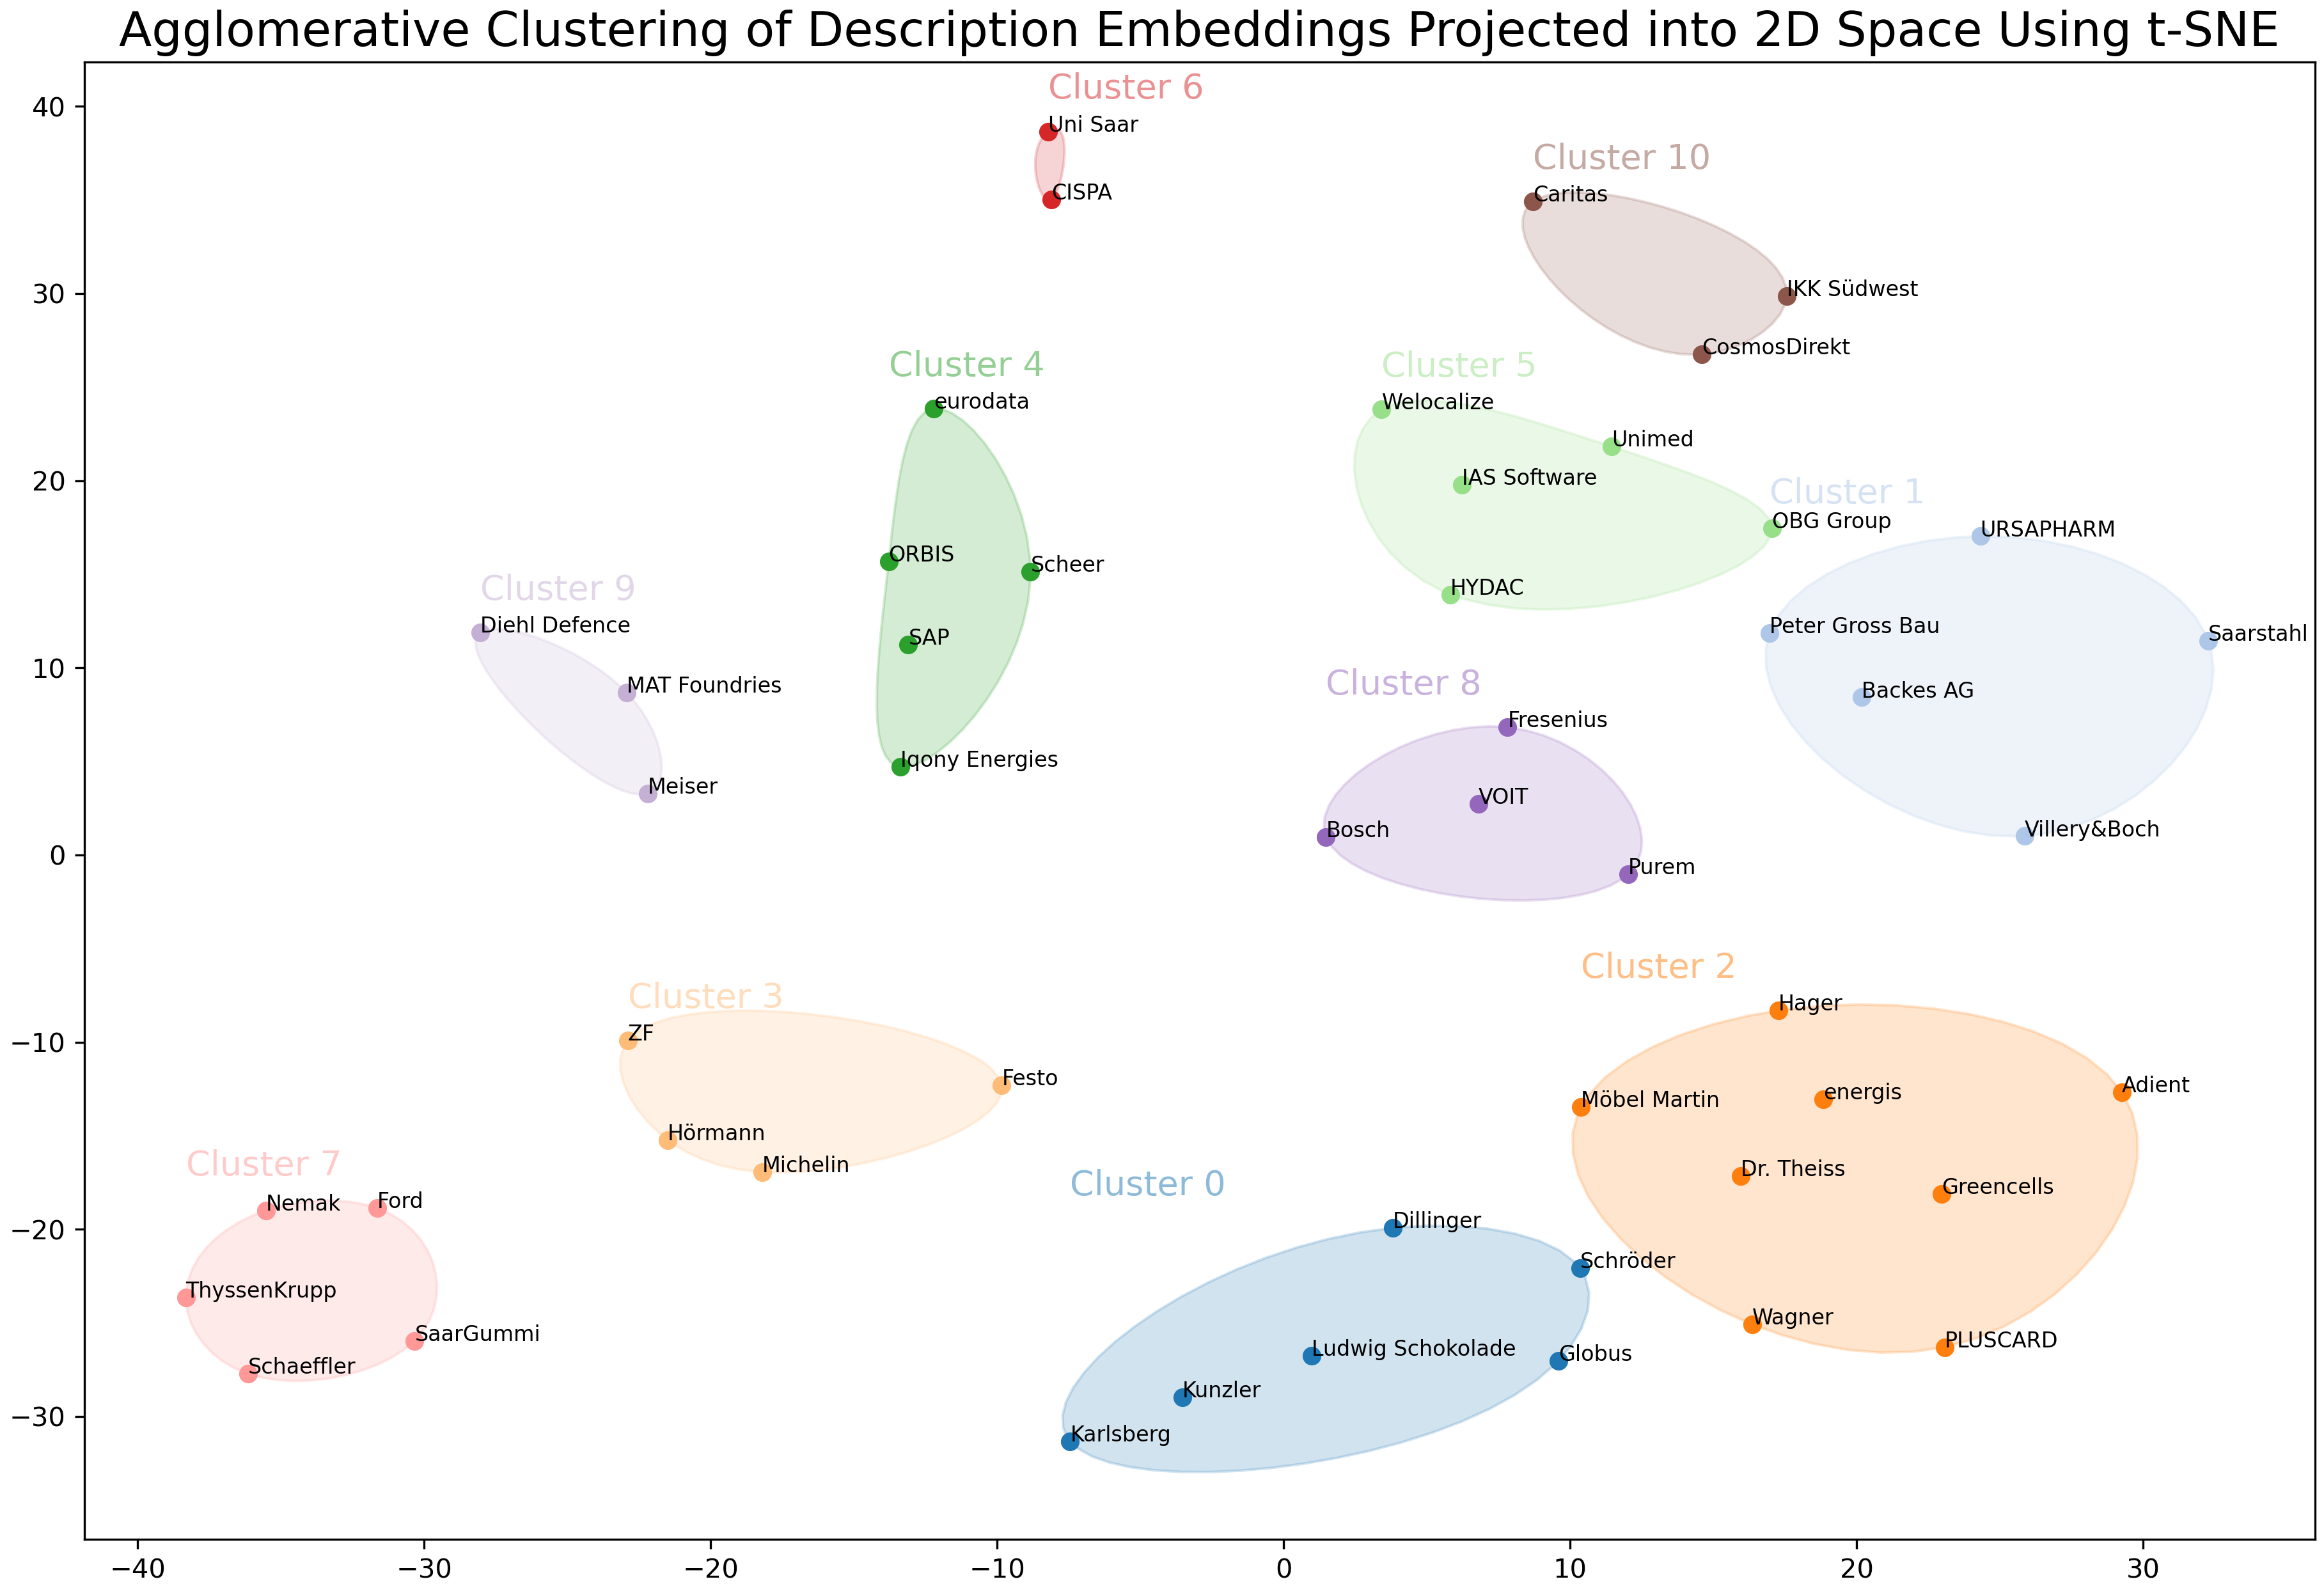
\includegraphics[width=0.5\textwidth]{figures/clustering_tsne.png}
    \caption{Clustering of company descriptions using t-SNE and Agglomerative clustering.}
    \label{fig:t-sne-agglomerative}
\end{figure}

In this section, we will investigate the results of the best-performing configuration of our clustering and location recommendation system. These results were obtained using the following configuration: the description embeddings were computed using max pooling, the embeddings were projected into 2D space using t-SNE, and the clustering was achieved using Agglomerative clustering. We found that this configuration yields the most sensible predictions of market segments and location recommendations. Figure \hyperref[fig:t-sne-agglomerative]{$2$} displays the resulting clustered data points, and the plots of the other configurations can be found in the appendix.

\subsection{Clustering}
In the following, we analyze each of the found clusters and interpret them with respect to potential market segments:
\begin{itemize}
    \item \textit{Cluster 0 (dark blue)}: This cluster contains the four large food producers Karlsberg, Kunzler, Ludwig Schokolade, and Schröder. Hence, we classify it as the food market segment. It also contains Globus, a large supermarket chain that also produces its own foods. The last member of this cluster is Dillinger, which we can discard as incorrectly assigned since it is a steel manufacturer.

    \item \textit{Cluster 1 (light blue)}: We cannot infer a market segment from the members of this cluster since it contains vastly different companies, such as the pharmaceutical company URSAPHARM, the ceramics manufacturer Villeroy\&Boch, and the steel manufacturer Saarstahl. However, it contains the construction companies Peter Gross Bau and Backes AG, and the OBG Group, which is assigned to Cluster $5$, is another construction company close to the first two companies. Hence, we follow that there is a construction market segment in Saarland.

    \item \textit{Cluster 2 (dark orange)}: The data points of this cluster have the largest relative distance due to them sharing no commonalities, and thus we cannot derive a potential market segment.

    \item \textit{Cluster 3 (light orange)}: The large automotive suppliers ZF and Michelin are part of this cluster, which explains its proximity to Cluster $7$ (automotive industry market segment). However, Hörmann, which produces doors for commercial and industrial applications, and Festo, which produces industrial automation systems, are also part of this cluster. Since the only commonality between these companies is that they are large, multi-national, industrial companies, we cannot assign them to a single market segment.

    \item \textit{Cluster 4 (dark green)}: The IT / IT consulting firms eurodata, ORBIS, Scheer, and SAP are part of this cluster, so we classify it as the IT consulting market segment. The fifth member of this cluster is Iqony Energies, which is seemingly misclassified since it provides energy solutions, yet it resembles the other cluster members since it also does consulting and IT infrastructure.

    \item \textit{Cluster 5 (light green)}: This cluster contains the companies Welocalize, Unimed, and IAS Software, which provide IT services such as document translation, accounting, and data collection. Hence, we follow that this cluster is representative of the IT service market segment. Note that the remaining two cluster members can be considered incorrectly assigned. HYDAC should be added to Cluster $7$ (automotive industry market segment), and OBG Group should be in a single cluster with Peter Gross Bau and Backes AG (construction market segment).

    \item \textit{Cluster 6 (dark red)}: The only two members of this cluster are Uni Saar and CISPA, making it representative of the academia market segment.

    \item \textit{Cluster 7 (light red)}: It corresponds to the automotive industry market segment since it comprises the automotive manufacturers and suppliers Nemak, Ford, ThyssenKrupp, Schaeffler, and SaarGummi.

    \item \textit{Cluster 8 (dark purple)}: This cluster contains Bosch, VOIT, Fresenius, and Purem, which focus on electrical engineerings, such as filtration systems and powertrain components for electric cars. Thus, this cluster corresponds to the electronics industry market segment.

    \item \textit{Cluster 9 (light purple)}: The companies MAT Foundries and Meiser, which specialize in steel products, are part of this cluster, and the last cluster member is the weapons manufacturer Diehl Defence. This suggests that this cluster represents the steel industry market segment, and we note that the companies Dillinger and Saarstahl should also be contained in it.

    \item \textit{Cluster $10$ (brown)}: This cluster consists of Caritas, IKK Südwest, and CosmosDirekt, and thus we classify it as the healthcare and insurance market segment.
\end{itemize}

\subsection{Location Recommendation}
To test our location recommendation system, we generated descriptions for four fictional German companies with vastly different characteristics:
\begin{itemize}
    \item \textit{FluxAI}: A young artificial intelligence start-up with ambitious goals of revolutionizing healthcare, finance, energy, and transportation.
    \item \textit{ABC Auto}: A well-established automotive manufacturer offering a wide range of cars focusing on sustainability.
    \item \textit{Bratwurst Bliss}: A hot dog manufacturer that values traditional sausage making and locally sourced ingredients.
    \item \textit{PanzerTech}: A weapons manufacturer with a wide spectrum of products, from armored vehicles to cybersecurity solutions.
\end{itemize}

For FluxAI, our system recommends placing the new site close to CISPA, which is sensible since CISPA is a world leader in information security research, which also includes artificial intelligence, and thus knowledge transfer between both companies could be highly beneficial. It also makes sense that our system did not recommend locating FluxAI near IT companies with a more commercial focus, like SAP, since they primarily work on existing technology instead of revolutionary innovations.
For ABC Auto, the location recommendation is to establish a new site close to VOIT, which specializes in manufacturing car components with a focus on hybrid and electric cars. Thus, placing ABC Auto near VOIT would allow ABC Auto to source parts for its hybrid and electric cars from a company nearby, leading to a more robust supply chain.
For Bratwurst Bliss, the system recommends settling near the meat producer Kunzler, which could lead to knowledge transfer regarding sausage making.
Lastly, our system recommends placing PanzerTech's new site close to Diehl Defence, corresponding to the only weapons manufacturer in our dataset. Hence, this shows that our system does not need a large number of samples from each market segment to give reasonable location recommendations.

We conclude that our location recommendation system can reliably identify companies in our dataset with similar characteristics to companies seeking to establish sites in Saarland and thus can be used to foster the development of business clusters.

\subsection{Limitations}
We observed in subsection \textit{A} that we could not derive corresponding market segments for a small number of clusters because the cluster members had too different characteristics. These companies mostly belonged to sectors that are underrepresented in our dataset, such as ceramics manufacturing and pharmaceutics, so we would likely achieve more concise cluster assignments if we added more companies from these sectors to our dataset.

Another reason for invalid cluster assignments could be that our utilized sentence transformer was not fine-tuned for company descriptions, so that it could have produced inaccurate embeddings for some descriptions. Further, projecting the embeddings into 2D space could also cause inaccurate cluster assignments due to a large loss of information. Projecting the embeddings into higher dimensions might avoid this information loss, yet it would likely complicate or prevent a user-friendly visualization of the clustering results. We note that we observed no benefits from projecting the embeddings into 3D space.


\section{Conclusion}
\begin{itemize}
	\item \textbf{Recapitulate the Objectives:} Begin by restating the main project objectives or questions that guided your study. This helps to remind the reader of the purpose and scope of your research \cite{sample-article}.
	\item \textbf{Summarize the Key Findings:} Provide a brief summary of the main findings from your study. Highlight the most important results and their implications. However, avoid repeating all the details presented in the Results section. Instead, focus on the key outcomes that directly address your research objectives \cite{sample-web}.
	\item \textbf{Future Research Suggestions:} Identify potential directions for future research based on the limitations or gaps identified in your study. Discuss areas that would benefit from additional investigation or areas where more data or different methodologies could provide deeper insights.
	\item \textbf{Final remarks:} Provide a concise and thoughtful closing statement that summarizes the overall significance of your research. Reflect on the importance of your study and its potential impact on the field. Consider the broader implications of your findings and emphasize the value of your research contribution.
\end{itemize}

\bibliographystyle{IEEEtran}
\bibliography{bibliography}

\appendix
\begin{itemize}
	\item \textbf{Link to Code}: Provide the link to your code repository. You can use any service to host your code (Github, gdrive etc.). The code should be running, accessible and all of your work must be reproducible. In case your code is not accessible or not in a working state, relevant number of points will be deducted.   
	\item \textbf{Link to Overleaf}: Add a link to the Overleaf project which contains all of the LaTex related files for this report.
	\item \textbf{Additional Figures}: Add any and all additional figures produced during you work with relevant explanations in the appendix.
\end{itemize}

\end{document}
